\section{Word Embedding: One-Hot vs. Dense Vectors}
\begin{frame}{}
    \LARGE Word Embedding: \textbf{One-Hot vs. Dense Vectors}
\end{frame}

\begin{frame}[allowframebreaks]{Integer Representation of Words}
    \foreach \i in {1,...,2} { % Integers from 1 to 5
        \begin{figure}
            \centering
            \includegraphics[height=0.8\textheight,width=1\textwidth,keepaspectratio]{images/vector-space/iteger-repr-\i.png}
        \end{figure}

        \framebreak
    }
\end{frame}

\subsection{One-Hot Encoding}
\begin{frame}[allowframebreaks]{One-hot vectors}
    \foreach \i in {1,...,3} { % Integers from 1 to 5
        \begin{figure}
            \centering
            \includegraphics[height=0.8\textheight,width=1\textwidth,keepaspectratio]{images/vector-space/one-hot-vector-\i.png}
        \end{figure}

        \framebreak
    }
\end{frame}

\begin{frame}{One-Hot Encoding}
    \begin{itemize}
        \item Each word is represented as a unique vector.
        \item Vector has 1 at one position, 0 elsewhere.
        \item \textbf{Problems:}
        \begin{itemize}
            \item High-dimensional and sparse.
            \item No semantic meaning or similarity captured.
        \end{itemize}
    \end{itemize}
\end{frame}

\subsection{Dense Embeddings}
\begin{frame}{Dense Embeddings}
    \begin{itemize}
        \item Vectors are learned from data.
        \item Low-dimensional (e.g., 100--300).
        \item Capture semantic relationships.
        \item Example: \texttt{"king"} $-$ \texttt{"man"} $+$ \texttt{"woman"} $\approx$ \texttt{"queen"}
    \end{itemize}
\end{frame}

\begin{frame}[allowframebreaks]{Meaning as vectors}
    \foreach \i in {1,...,2} { % Integers from 1 to 5
        \begin{figure}
            \centering
            \includegraphics[height=0.8\textheight,width=1\textwidth,keepaspectratio]{images/vector-space/vector-meaning-\i.png}
        \end{figure}

        \framebreak
    }
\end{frame}

\begin{frame}[allowframebreaks]{Word embedding vectors}
    \begin{figure}
        \centering
        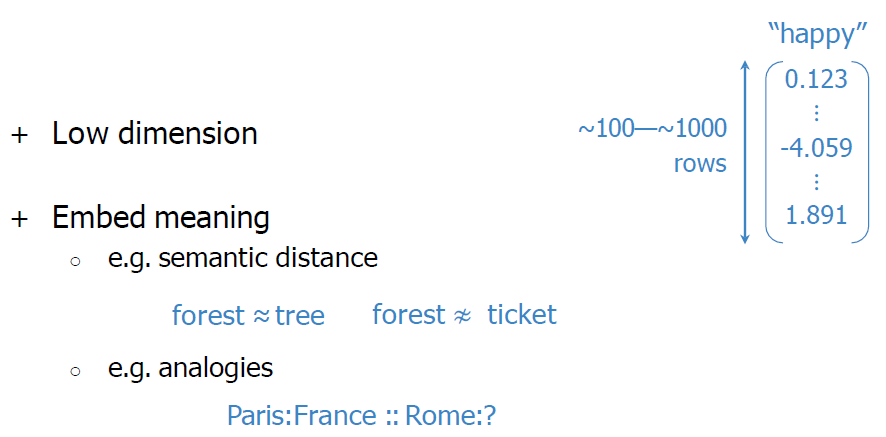
\includegraphics[width=\textwidth,height=0.65\textheight,keepaspectratio]{images/vector-space/word-embed-vec.png}
    \end{figure}
\end{frame}

\begin{frame}[allowframebreaks]{Terminology}
    \begin{figure}
        \centering
        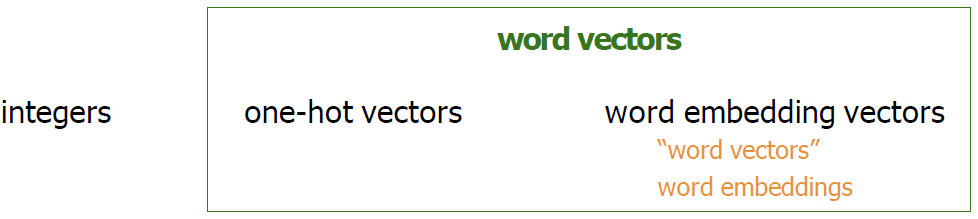
\includegraphics[width=\textwidth,height=0.65\textheight,keepaspectratio]{images/vector-space/terminology.png}
    \end{figure}
\end{frame}

\begin{frame}[allowframebreaks]{Word embedding process}
    \begin{figure}
        \centering
        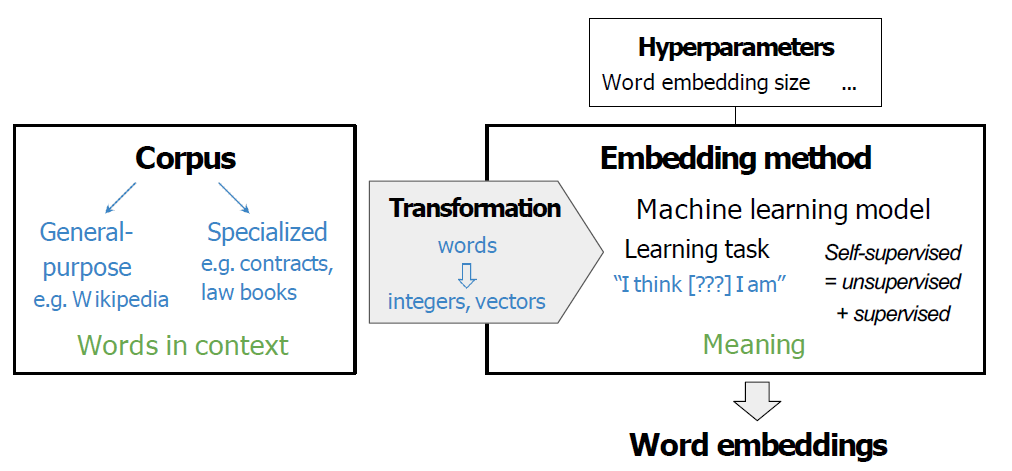
\includegraphics[width=\textwidth,height=0.8\textheight,keepaspectratio]{images/vector-space/word-embed-proc.png}
    \end{figure}
\end{frame}
